\documentclass[11pt,a4paper]{article}
\usepackage[utf8]{inputenc}
\usepackage{amsmath,amssymb,amsthm}
\usepackage{geometry}
\usepackage{booktabs}
\usepackage{tabularx}
\usepackage{hyperref}
\usepackage{microtype}
\usepackage{tikz}
\usepackage{pgfplots}
\pgfplotsset{compat=1.18}
\usetikzlibrary{arrows,positioning,shapes.geometric,calc}

\geometry{margin=1in}

\hypersetup{
    colorlinks=true,
    linkcolor=blue,
    citecolor=blue,
    urlcolor=blue,
    pdftitle={Deep Dive: Theorem B' --- Bayes Error \& Information Scaling},
    pdfauthor={Arben Lila}
}

\usepackage[firstpage=false]{draftwatermark}
\DraftwatermarkOptions{text={SUPERSEDED DRAFT\\DO NOT CITE},color=red!25,angle=55,scale=1.2}

\newtheorem{theorem}{Theorem}
\newtheorem{lemma}[theorem]{Lemma}
\newtheorem{definition}{Definition}
\newtheorem{claim}[theorem]{Claim}

\title{\textbf{A Pedagogical Deep Dive into Theorem $B'$}\\
\large Bayes Error and Information Scaling under $N \cdot I^2$ in the DAVID/M0.1 Engine}
\author{\textbf{Arben Lila} \\ \textit{Internal Thesis Work}}
\date{\today}

\begin{document}

\maketitle

\begin{abstract}
This report presents a mathematically rigorous and pedagogical deep dive into Theorem $B'$ (Bayes Error and Information Scaling). We analyze the information-theoretic boundaries of binary observation channels with low informativeness $I = |\rho - \delta|$. We prove two key results: (i) Theorem $B'.1$, which bounds the minimum classification error rate of a single observation to $\frac{1}{2}(1-I)$; and (ii) Theorem $B'.2$, which shows that the Fisher information scales as $N \cdot I^2$. We discuss the operational implications of the quadratic collapse of information as $I \to 0$, verify the results using pgfplots diagrams, and outline the engine's gatekeeper logic designed to protect conditional forecasts from prior domination.
\end{abstract}

\tableofcontents
\newpage

\section{Introduction \& The Information Limit}
A common pitfall in predictive policy modeling is overestimating the utility of noisy data sources. In the monitoring of Tobacco Industry (TI) tactics, observations are drawn from channels with unknown and often poor signal-to-noise ratios. If a scraper or coder is barely better than a coin flip, how much information does it actually provide about the latent activity state $A \in \{0, 1\}$?

Theorem $B'$ formalizes the absolute mathematical limits of such channels. It answers two crucial questions:
\begin{enumerate}
    \item What is the best classification accuracy any decision rule can achieve from a single noisy observation?
    \item How does our capacity to estimate the prevalence $\phi$ of the latent state scale as the source informativeness vanishes, and how many samples $N$ are required to compensate?
\end{enumerate}

By understanding these bounds, we can build a predictive engine that mathematically refuses to emit point forecasts for cells that do not meet the necessary information-theoretic floor.

---

\section{Parameter Glossary}
Table~\ref{tab:parameters} lists the mathematical symbols, domains, and operational interpretations for Theorem $B'$.

\begin{table}[h]
\centering
\caption{Parameter definitions and domains for the Theorem $B'$ analysis.}
\label{tab:parameters}
\begin{tabularx}{\textwidth}{llX}
\toprule
\textbf{Symbol} & \textbf{Domain} & \textbf{Operational Interpretation} \\
\midrule
$A \in \{0, 1\}$ & Latent state space & True underlying presence of a TI tactic class. \\
$Y \in \{0, 1\}$ & Observed state space & Binary label output from a source or coder. \\
$\phi \in [0, 1]$ & Parameter space & True marginal probability $P(A = 1)$. \\
$\rho \in [0, 1]$ & Channel Parameter & Sensitivity (True Positive Rate) $P(Y = 1 \mid A = 1)$. \\
$\delta \in [0, 1]$ & Channel Parameter & False Positive Rate $P(Y = 1 \mid A = 0)$. \\
$I \in [0, 1]$ & Channel Informativeness & Channel signal strength: $I = |\rho - \delta|$. \\
$\varepsilon^\star \in [0, 0.5]$ & Error bound & Minimum probability of classification error (Bayes error). \\
$I_F(\phi) \in [0, \infty)$ & Information measure & Fisher Information of the prevalence parameter $\phi$. \\
\bottomrule
\end{tabularx}
\end{table}

---

\section{Theorem $B'.1$ --- Single-Observation Bayes Error}

\subsection{Formal Statement}
\begin{theorem}[Single-Observation Bayes Error]
Under equal prior odds ($P(A=1) = 0.5$), the minimum classification error rate $\varepsilon^\star$ for recovering the latent state $A$ from a single binary observation $Y$ is:
\begin{equation}\label{eq:bayes_error_bound}
\varepsilon^\star = \frac{1}{2}(1 - I)
\end{equation}
where $I = |\rho - \delta|$ is the channel informativeness.
\end{theorem}

\subsection{Proof}
\begin{proof}
Let $g(Y) \in \{0, 1\}$ be any decision rule (classifier) mapping the observed label $Y$ to an estimate of the latent state $A$. The probability of classification error is:
\[
P(\text{Error}) = P(g(Y) \neq A)
\]
Under equal priors ($P(A=1) = P(A=0) = 0.5$), the minimum error probability is achieved by the MAP (Maximum A Posteriori) decision rule, which is the Bayes classifier. The Bayes error $\varepsilon^\star$ is given by:
\[
\varepsilon^\star = \frac{1}{2} \left( 1 - \text{TV}(P_{Y \mid A=1}, P_{Y \mid A=0}) \right)
\]
where $\text{TV}$ is the Total Variation distance between the two class-conditional probability laws of $Y$. Since $Y$ is a binary random variable, $P_{Y \mid A=1} \sim \text{Bernoulli}(\rho)$ and $P_{Y \mid A=0} \sim \text{Bernoulli}(\delta)$. 

We compute the Total Variation distance:
\begin{align*}
    \text{TV}(P_{Y \mid A=1}, P_{Y \mid A=0}) &= \frac{1}{2} \sum_{y \in \{0, 1\}} |P(Y=y \mid A=1) - P(Y=y \mid A=0)| \\
    &= \frac{1}{2} \left( |P(Y=1 \mid A=1) - P(Y=1 \mid A=0)| + |P(Y=0 \mid A=1) - P(Y=0 \mid A=0)| \right) \\
    &= \frac{1}{2} \left( |\rho - \delta| + |(1 - \rho) - (1 - \delta)| \right) \\
    &= \frac{1}{2} \left( |\rho - \delta| + |\delta - \rho| \right) \\
    &= |\rho - \delta| = I
\end{align*}
Substituting $\text{TV} = I$ into the Bayes error equation:
\[
\varepsilon^\star = \frac{1}{2}(1 - I)
\]
This completes the proof. Any classifier trying to predict $A$ using only $Y$ must suffer an error rate of at least $\frac{1}{2}(1 - I)$.
\end{proof}

\subsection{Visual Representation}
Figure~\ref{fig:bayes_error} displays the linear relationship between informativeness and the Bayes error bound. If $I = 0$ (a completely uninformative channel), the minimum error is $\varepsilon^\star = 0.50$, equivalent to random guessing. Only when $I = 1$ (a perfect, noiseless channel) can the error rate reach $0$.

\begin{figure}[htbp]
\centering
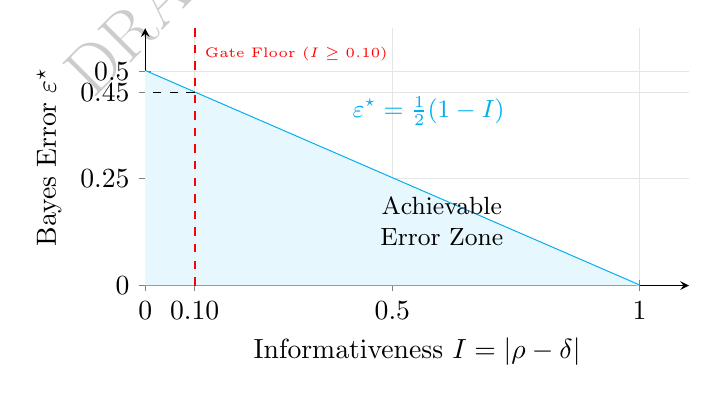
\begin{tikzpicture}
\begin{axis}[
    width=0.7\textwidth,
    height=0.4\textwidth,
    axis lines=left,
    xlabel={Informativeness $I = |\rho - \delta|$},
    ylabel={Bayes Error $\varepsilon^\star$},
    xmin=0, xmax=1.1,
    ymin=0, ymax=0.6,
    xtick={0, 0.1, 0.5, 1},
    xticklabels={0, $0.10$, 0.5, 1},
    ytick={0, 0.25, 0.45, 0.5},
    yticklabels={0, 0.25, $0.45$, 0.5},
    grid=both,
    grid style={line width=.1pt, draw=gray!10},
    major grid style={line width=.2pt, draw=gray!20},
]
\addplot[thick, cyan, domain=0:1] {0.5*(1 - x)};
\addplot[fill=cyan!10, draw=none, domain=0:1] {0.5*(1 - x)} \closedcycle;
\node[anchor=south west, text=cyan, font=\small] at (axis cs: 0.4, 0.35) {$\varepsilon^\star = \frac{1}{2}(1 - I)$};

% Draw Gate Floor
\draw[dashed, red, thick] (axis cs: 0.1, 0) -- (axis cs: 0.1, 0.6) node[pos=0.9, right, font=\tiny] {Gate Floor ($I \ge 0.10$)};
\draw[dashed, black] (axis cs: 0.1, 0.45) -- (axis cs: 0, 0.45);
\node[anchor=east, font=\tiny, text=red] at (axis cs: 0, 0.45) {Max Allowable Error ($0.45$)};

\node[align=center, font=\small] at (axis cs: 0.6, 0.15) {Achievable\\Error Zone};
\end{axis}
\end{tikzpicture}
\caption{Bayes error rate $\varepsilon^\star$ plotted against informativeness $I$. The red dashed line denotes the information floor of $0.10$, corresponding to a maximum allowable classification error of $45\%$.}
\label{fig:bayes_error}
\end{figure}

---

\section{Theorem $B'.2$ --- Asymptotic Information Scaling}

\subsection{Formal Statement}
\begin{theorem}[Information Scaling]
Let $Y_1, \dots, Y_N$ be $N$ conditionally independent binary observations from a channel with parameters $\rho, \delta$ and informativeness $I = |\rho - \delta|$. The Fisher information $I_F(\phi)$ of the latent prevalence parameter $\phi$ scales quadratically with $I$:
\begin{equation}\label{eq:fisher_info_scaling}
I_F(\phi) = N \frac{I^2}{p(1 - p)}
\end{equation}
where $p = P(Y=1) = \delta + \phi(\rho - \delta)$ is the marginal probability of a positive observation.
\end{theorem}

\subsection{Proof}
\begin{proof}
Let $Y \sim \text{Bernoulli}(p)$ be a single binary observation. Assuming without loss of generality that $\rho > \delta$, the success probability is:
\[
p = \delta + \phi(\rho - \delta) = \delta + I\phi
\]
The probability mass function of $Y$ is:
\[
f(y \mid \phi) = p^y (1 - p)^{1 - y}
\]
Taking the natural logarithm:
\[
\ln f(y \mid \phi) = y \ln(p) + (1 - y) \ln(1 - p)
\]
We compute the score function by taking the partial derivative with respect to $\phi$:
\[
\frac{\partial}{\partial \phi} \ln f(y \mid \phi) = y \frac{1}{p} \frac{\partial p}{\partial \phi} - (1 - y) \frac{1}{1 - p} \frac{\partial p}{\partial \phi}
\]
Since $\frac{\partial p}{\partial \phi} = \frac{\partial}{\partial \phi} (\delta + I\phi) = I$:
\[
\frac{\partial}{\partial \phi} \ln f(y \mid \phi) = I \left( \frac{y}{p} - \frac{1 - y}{1 - p} \right) = I \frac{y - p}{p(1 - p)}
\]
The Fisher information of a single observation is the variance of the score function:
\begin{align*}
    I_{F, 1}(\phi) &= E\left[ \left( \frac{\partial}{\partial \phi} \ln f(Y \mid \phi) \right)^2 \right] \\
    &= E\left[ \frac{I^2 (Y - p)^2}{p^2 (1 - p)^2} \right] \\
    &= \frac{I^2}{p^2 (1 - p)^2} E[(Y - p)^2]
\end{align*}
Since $Y \sim \text{Bernoulli}(p)$, its variance is $E[(Y - p)^2] = p(1-p)$. Substituting this in:
\[
I_{F, 1}(\phi) = \frac{I^2}{p^2 (1 - p)^2} p(1 - p) = \frac{I^2}{p(1 - p)}
\]
By the additivity of Fisher information for $N$ conditionally independent observations, the total Fisher information is:
\[
I_F(\phi) = N \cdot I_{F, 1}(\phi) = N \frac{I^2}{p(1 - p)}
\]
This completes the proof.
\end{proof}

\subsection{The Quadratic Collapse ($I \to 0$)}
The denominator $p(1 - p)$ represents the variance of the observed data and is bounded by $0.25$ (achieved when $p = 0.5$). Thus, we establish the inequality:
\begin{equation}\label{eq:scaling_bound}
I_F(\phi) \ge 4 N \cdot I^2
\end{equation}

As the informativeness $I$ vanishes, the Fisher information collapses **quadratically**. By the Cramer-Rao bound, the variance of any unbiased estimator $\hat{\phi}$ is bounded by the reciprocal of the Fisher information:
\[
\text{Var}(\hat{\phi}) \ge \frac{1}{I_F(\phi)} \approx \frac{p(1-p)}{N \cdot I^2}
\]
To maintain a constant estimation precision $\sigma^2 = \text{Var}(\hat{\phi})$, the required sample size scales as:
\[
N \propto \frac{1}{I^2}
\]
If a source's informativeness drops by a factor of 10 (e.g., from $0.50$ to $0.05$), you need **100 times more data** ($10^2$) to achieve the same confidence. 

Figure~\ref{fig:info_scaling} illustrates this behavior across different sample sizes. It shows that for low informativeness ($I < 0.10$), even large sample sizes ($N = 100$) yield negligible information about the latent state.

\begin{figure}[htbp]
\centering
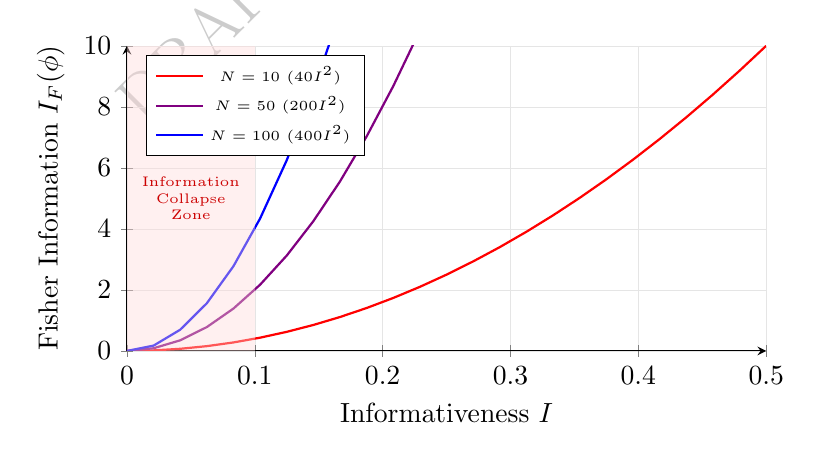
\begin{tikzpicture}
\begin{axis}[
    width=0.8\textwidth,
    height=0.45\textwidth,
    axis lines=left,
    xlabel={Informativeness $I$},
    ylabel={Fisher Information $I_F(\phi)$},
    xmin=0, xmax=0.5,
    ymin=0, ymax=10,
    xtick={0, 0.1, 0.2, 0.3, 0.4, 0.5},
    ytick={0, 2, 4, 6, 8, 10},
    grid=both,
    grid style={line width=.1pt, draw=gray!10},
    major grid style={line width=.2pt, draw=gray!20},
    legend pos=north west,
    legend style={font=\tiny},
]
\addplot[thick, red, domain=0:0.5] {4*10*x^2};
\addlegendentry{$N=10$ ($40 I^2$)}
\addplot[thick, violet, domain=0:0.5] {4*50*x^2};
\addlegendentry{$N=50$ ($200 I^2$)}
\addplot[thick, blue, domain=0:0.5] {4*100*x^2};
\addlegendentry{$N=100$ ($400 I^2$)}

% Shading the uninformative region
\fill[red!15, opacity=0.4] (axis cs: 0,0) rectangle (axis cs: 0.1,10);
\node[text=red!80!black, font=\tiny, align=center] at (axis cs: 0.05, 5) {Information\\Collapse\\Zone};

\end{axis}
\end{tikzpicture}
\caption{Fisher information $I_F(\phi)$ as a function of informativeness $I$ for various sample sizes $N$ (assuming worst-case $p(1-p)=0.25$). The red shaded zone highlights the region of information collapse where Gate FG3 enforces a block.}
\label{fig:info_scaling}
\end{figure}

---

\section{System Enforcement (Gate FG3)}
The DAVID/M0.1 engine guards against information collapse by checking the lower credible bound of informativeness. 
* **Computation:** During MCMC sampling, the posterior draws of the source parameters $\rho_s$ and $\delta_s$ are extracted. For each cell, the engine computes:
  \[
  I = |\rho_s - \delta_s|
  \]
* **Operational Gate (FG3):** The forecast passes only if:
  \[
  I_{\text{lower 95\%}} \ge \text{INFORMATIVENESS\_FLOOR\_LOWER\_95} = 0.10
  \]
* **Fail-Closed Action:** If the lower bound falls below $0.10$, the cell's forecast route is degraded to \texttt{prior\_dominated}. The dashboard automatically hides the conditional point forecast and displays a wide prior interval instead, protecting users from trusting uninformative data.

\end{document}
